\documentclass[11pt,a4paper]{article}
\usepackage[T1]{fontenc}
\usepackage[utf8]{inputenc}
\usepackage{lmodern}
\usepackage{amsmath,amssymb,amsthm,mathtools,mathrsfs}
\usepackage{graphicx,float,xcolor,multicol}
\usepackage[shortlabels]{enumitem}
\usepackage[margin=27mm]{geometry}
\usepackage{microtype,needspace,placeins}
\usepackage{tikz,tikz-cd}
\usetikzlibrary{arrows.meta,calc,positioning,patterns,decorations.pathreplacing}
\usepackage[colorlinks=true,linkcolor=teal,urlcolor=teal,citecolor=teal]{hyperref}
\setlength{\parindent}{0pt}
\setlength{\parskip}{.6em}
\setcounter{secnumdepth}{0}
\allowdisplaybreaks
\raggedbottom
\providecommand{\cross}{\times}
\DeclareUnicodeCharacter{2020}{\ensuremath{\dagger}}
\DeclareMathOperator{\supp}{supp}
\DeclareMathOperator*{\esssup}{ess\,sup}
\providecommand{\chapter}{\section}
\newenvironment{tool}[2]{\subsection*{Tool #1 --- #2}}{}
\newcommand{\ToolRef}[1]{Tool #1}
\newcommand{\FigureTag}[2]{\textit{Figure #1}}
\newcommand{\Result}[1]{\subsection*{#1}}
\newcommand{\Application}[1]{\subsubsection*{Application\if\relax\detokenize{#1}\relax\else\space--- #1\fi}}
\newcommand{\ProofHeading}{\par\textit{Proof.}\space}
\newcommand{\ProofOf}[1]{\par\textit{Proof of #1.}\space}
\newcommand{\RemarkHeading}{\par\textbf{Remark.}\space}
\newcommand{\NoteHeading}{\par\textbf{Note.}\space}
\newcommand{\ExerciseHeading}{\par\textbf{Exercise.}\space}

% Rendering support only; mathematical text is in each independent post.
\usepackage{booktabs,array,longtable}
\definecolor{HandoutBlue}{HTML}{2F6690}
\definecolor{HandoutNavy}{HTML}{17365D}
\newtheorem{theorem}{Theorem}
\newtheorem{lemma}[theorem]{Lemma}
\newtheorem{proposition}[theorem]{Proposition}
\newtheorem{corollary}[theorem]{Corollary}
\newtheorem{conjecture}[theorem]{Conjecture}
\newtheorem{definition}{Definition}
\newtheorem{example}{Example}
\newtheorem{namedtoolcounter}{Tool}
\newenvironment{namedtool}[1]{\begin{namedtoolcounter}[#1]}{\end{namedtoolcounter}}
\newtheorem*{claim}{Claim}
\newtheorem*{remark}{Remark}
\newtheorem*{exercise}{Exercise}
\newtheorem*{question}{Question}
\newtheorem*{observation}{Observation}
\newcommand{\SourceChapter}[2]{\section*{#2}}
\newcommand{\Lecture}[2]{\section*{Lecture #1: #2}}
\newcommand{\unclear}[1]{\textit{[unclear: #1]}}
\newcommand{\sourcegap}{\textit{[unfinished in the source]}}
\DeclareMathOperator{\dist}{dist}
\DeclareMathOperator{\id}{id}
\DeclareMathOperator{\Hol}{Hol}
\DeclareMathOperator{\Per}{Per}
\DeclareMathOperator{\Fix}{Fix}
\DeclareMathOperator{\diam}{diam}
\DeclareMathOperator{\Var}{Var}
\DeclareMathOperator{\Leb}{Leb}
\DeclareMathOperator{\Hom}{Hom}
\DeclareMathOperator{\End}{End}
\DeclareMathOperator{\Ann}{Ann}
\DeclareMathOperator{\Spec}{Spec}
\DeclareMathOperator{\Max}{Max}
\DeclareMathOperator{\Ob}{Ob}
\DeclareMathOperator{\Tor}{Tor}
\DeclareMathOperator{\Ass}{Ass}
\DeclareMathOperator{\Mor}{Mor}
\DeclareMathOperator{\Fun}{Fun}
\DeclareMathOperator{\Nat}{Nat}
\DeclareMathOperator{\Cone}{Cone}
\DeclareMathOperator{\MCG}{MCG}
\DeclareMathOperator{\Aut}{Aut}
\DeclareMathOperator{\Deck}{Deck}
\DeclareMathOperator{\SL}{SL}
\DeclareMathOperator{\PSL}{PSL}
\DeclareMathOperator{\Area}{Area}
\DeclareMathOperator{\im}{im}
\DeclareMathOperator{\PSh}{PSh}
\newcommand{\CRing}{\mathsf{CRings}}
\newcommand{\AMod}{A\text{-}\mathsf{Mod}}
\newcommand{\Ab}{\mathsf{Ab}}
\newcommand{\Z}{\mathbb Z}
\newcommand{\Q}{\mathbb Q}
\newcommand{\R}{\mathbb R}
\newcommand{\C}{\mathbb C}
\newcommand{\N}{\mathbb N}
\newcommand{\kk}{\mathbb k}
\renewcommand{\aa}{\mathfrak a}
\newcommand{\bb}{\mathfrak b}
\newcommand{\pp}{\mathfrak p}
\newcommand{\qq}{\mathfrak q}
\newcommand{\mm}{\mathfrak m}
\newcommand{\nn}{\mathfrak n}
\newcommand{\rad}{\mathrm r}
\newcommand{\cat}[1]{\mathsf{#1}}
\setcounter{secnumdepth}{0}
\allowdisplaybreaks

% Notation used only by the newly added notes.
\setlength{\emergencystretch}{2em}
\providecommand{\D}{\mathbb D}
\providecommand{\M}{\mathcal M}
\providecommand{\Chat}{\widehat{\mathbb C}}
\providecommand{\Crit}{\operatorname{Crit}}
\providecommand{\Int}{\operatorname{Int}}
\providecommand{\Ext}{\operatorname{Ext}}

\graphicspath{{figures/quadratic-family/}}
\begin{document}
\section*{Conformal Welding}
% BLOG-CONTENT-BEGIN
% Source page 14
\subsection{Simultaneous uniformisation of Blaschke products}
Consider expanding finite Blaschke products. Given two Blaschke products $B_1,B_2$ of degree $d$, each $B_i$ is a rational map of degree $d$. If $B_i$ is expanding on its Julia set, then $B_i$ is hyperbolic, and
\[
B_i(\D)=\D,
\qquad B_i(\Chat\setminus\overline\D)=\Chat\setminus\overline\D.
\]
By Montel's theorem, $J(B_i)=S^1$. Thus $B_i\colon S^1\to S^1$ is a $d$-fold cover.

Since each restriction $B_i|_{S^1}$ is a real-analytic expanding orientation-preserving covering of degree $d$, the quasisymmetric classification of expanding circle maps gives a quasisymmetric homeomorphism $\psi:S^1\to S^1$ such that $\psi\circ B_1|_{S^1}\circ\psi^{-1}=B_2|_{S^1}$.

% Source page 15
Given $\psi\circ B_1\circ\psi^{-1}=B_2$, with $\psi$ quasisymmetric, can we realize $\psi$ as $\widetilde R_V\circ\widetilde R_U^{-1}$, where $\widetilde R_V,\widetilde R_U$ are extensions of Riemann maps to the boundary?

We have a quasisymmetric map $\psi\colon S^1\to S^1$. Extend it to a quasiconformal map $\widehat\psi\colon\overline\D\to\overline\D$. Set
\[
\mu:=\begin{cases}
(\widehat\psi^{-1})^*\mu_0,&\text{on }\D,\\
\mu_0,&\text{on }\Chat\setminus\overline\D.
\end{cases}
\]
Let $\phi$ be an integrating map for $\mu$. Then
\[
\begin{aligned}
(\phi\circ\widehat\psi)^*\mu_0
 &=\widehat\psi^*(\phi^*(\mu_0))=\mu_0
 &&\text{on }\D,\\
\phi^*(\mu_0)&=\mu_0
 &&\text{on }\Chat\setminus\overline\D.
\end{aligned}
\]
Consequently, the maps
\[
\begin{aligned}
\phi\circ\widehat\psi&\colon(\D,\mu_0)\longrightarrow(\phi(\D),\mu_0),\\
\phi&\colon(\Chat\setminus\overline\D,\mu_0)
 \longrightarrow(\phi(\Chat\setminus\overline\D),\mu_0)
\end{aligned}
\]
are conformal. The curve $\gamma=\phi(S^1)$ is a quasicircle. Set $U=\phi(\D)$ and $V=\phi(\Chat\setminus\overline\D)$. Set
\[
\widetilde R_U=(\phi\circ\widehat\psi)^{-1}\colon U\to\D,
\qquad
\widetilde R_V=\phi^{-1}\colon V\to\Chat\setminus\overline\D.
\]

The map $\psi$ is called a \emph{conformal welding} of $\gamma$.

The following diagram records the domains and boundary identifications needed for the welding.
\begin{figure}[H]
\centering
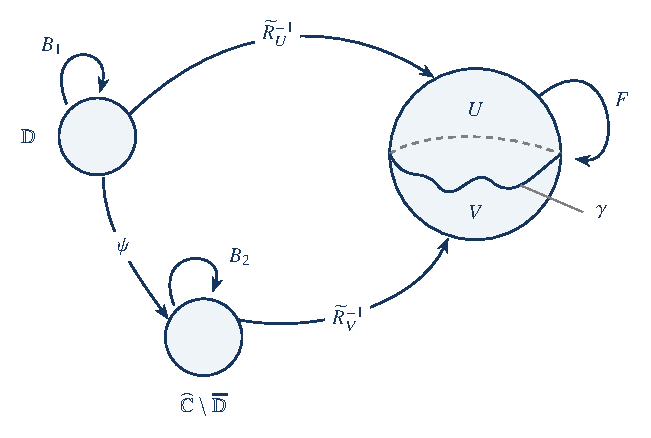
\includegraphics[width=11.8cm,height=6.6cm,keepaspectratio]{qf-fig-08.pdf}
\FigureTag{QF8}{fig:qf-08}
\end{figure}
Then we can define
\[
F(z)=\begin{cases}
\widetilde R_U^{-1}\circ B_1\circ\widetilde R_U(z),&z\in\overline U,\\
\widetilde R_V^{-1}\circ B_2\circ\widetilde R_V(z),&z\in\overline V.
\end{cases}
\]
On $\gamma$, we have $F=\widetilde R_U^{-1}\circ B_1\circ\widetilde R_U
 =\widetilde R_V^{-1}\circ B_2\circ\widetilde R_V$.
Therefore, on $S^1$, $(\widetilde R_V\circ\widetilde R_U^{-1})\circ B_1
\circ(\widetilde R_U\circ\widetilde R_V^{-1})=B_2$.
% BLOG-CONTENT-END
\end{document}
